\documentclass[a4paper, 12pt]{extarticle}

\usepackage{arxiv}

\usepackage[T2A]{fontenc}
\usepackage[utf8]{inputenc}
\usepackage[english, russian]{babel}
% \usepackage{cmap}
\usepackage{url}
\usepackage{booktabs}
\usepackage{nicefrac}
\usepackage{microtype}
\usepackage{lipsum}
\usepackage{graphicx}
\usepackage{epstopdf}
\usepackage{subfig}
\usepackage[square,sort,comma,numbers]{natbib}
\usepackage{doi}
\usepackage{multicol}
\usepackage{multirow}
\usepackage{tabularx}
\usepackage{float}
\usepackage{amssymb}

\usepackage{tikz}
\usetikzlibrary{matrix}

% Algorithms
\usepackage{algpseudocode}
\usepackage{algorithm}

%% Шрифты
\usepackage{euscript} % Шрифт Евклид
\usepackage{mathrsfs} % Красивый матшрифт
\usepackage{extsizes} % Возможность сделать 14-й шрифт
\usepackage{bm}

\usepackage{makecell} % diaghead in a table
\usepackage{amsmath,amsfonts,amssymb,amsthm,mathtools,dsfont}
\usepackage{icomma}
\usepackage[labelfont=bf]{caption}
\usepackage{subfig} % for subfigures
\usepackage{wrapfig}

\newcommand{\bz}{\mathbf{z}}
\newcommand{\bx}{\mathbf{x}}
\newcommand{\by}{\mathbf{y}}
\newcommand{\bv}{\mathbf{v}}
\newcommand{\bw}{\mathbf{w}}
\newcommand{\ba}{\mathbf{a}}
\newcommand{\bb}{\mathbf{b}}
\newcommand{\bp}{\mathbf{p}}
\newcommand{\bq}{\mathbf{q}}
\newcommand{\bt}{\mathbf{t}}
\newcommand{\bu}{\mathbf{u}}
\newcommand{\bs}{\mathbf{s}}
\newcommand{\bT}{\mathbf{T}}
\newcommand{\bX}{\mathbf{X}}
\newcommand{\bZ}{\mathbf{Z}}
\newcommand{\bS}{\mathbf{S}}
\newcommand{\bH}{\mathbf{H}}
\newcommand{\bW}{\mathbf{W}}
\newcommand{\bY}{\mathbf{Y}}
\newcommand{\bU}{\mathbf{U}}
\newcommand{\bQ}{\mathbf{Q}}
\newcommand{\bP}{\mathbf{P}}
\newcommand{\bA}{\mathbf{A}}
\newcommand{\bB}{\mathbf{B}}
\newcommand{\bC}{\mathbf{C}}
\newcommand{\bE}{\mathbf{E}}
\newcommand{\bF}{\mathbf{F}}
\newcommand{\bomega}{\boldsymbol{\omega}}
\newcommand{\btheta}{\boldsymbol{\theta}}
\newcommand{\bgamma}{\boldsymbol{\gamma}}
\newcommand{\bdelta}{\boldsymbol{\delta}}
\newcommand{\bPsi}{\boldsymbol{\Psi}}
\newcommand{\bpsi}{\boldsymbol{\psi}}
\newcommand{\bxi}{\boldsymbol{\xi}}
\newcommand{\bchi}{\boldsymbol{\chi}}
\newcommand{\bzeta}{\boldsymbol{\zeta}}
\newcommand{\blambda}{\boldsymbol{\lambda}}
\newcommand{\beps}{\boldsymbol{\varepsilon}}
\newcommand{\bZeta}{\boldsymbol{Z}}
% mathcal
\newcommand{\cX}{\mathcal{X}}
\newcommand{\cY}{\mathcal{Y}}
\newcommand{\cW}{\mathcal{W}}

\newcommand{\dH}{\mathds{H}}
\newcommand{\dR}{\mathds{R}}
% transpose
\newcommand{\T}{^{\mathsf{T}}}

% \renewcommand{\shorttitle}{\textit{arXiv} Шаблон}
\renewcommand{\epsilon}{\ensuremath{\varepsilon}}
\renewcommand{\phi}{\ensuremath{\varphi}}
\renewcommand{\kappa}{\ensuremath{\varkappa}}
\renewcommand{\le}{\ensuremath{\leqslant}}
\renewcommand{\leq}{\ensuremath{\leqslant}}
\renewcommand{\ge}{\ensuremath{\geqslant}}
\renewcommand{\geq}{\ensuremath{\geqslant}}
\renewcommand{\emptyset}{\varnothing}

\DeclareMathOperator*{\argmax}{arg\,max}  % in your preamble
\DeclareMathOperator*{\argmin}{arg\,min}  % in your preamble 

\usepackage{hyperref}
% \usepackage[usenames,dvipsnames,svgnames,table,rgb]{xcolor}

\hypersetup{
	unicode=true,
	pdftitle={A template for the arxiv style},
	pdfsubject={q-bio.NC, q-bio.QM},
	pdfauthor={David S.~Hippocampus, Elias D.~Striatum},
	pdfkeywords={First keyword, Second keyword, More},
	colorlinks=true,
	linkcolor=black,        % внутренние ссылки
	citecolor=blue,         % на библиографию
	filecolor=magenta,      % на файлы
	urlcolor=blue           % на URL
}

\graphicspath{{./figures}}

\usepackage{enumitem} % Для модификаций перечневых окружений

\theoremstyle{definition} % "Определение"
\newtheorem{definition}{Опр.}[section]

\usepackage{etoolbox}

\makeatletter
\expandafter\patchcmd\csname\string\algorithmic\endcsname{\itemsep\z@}{\itemsep=1.5mm}{}{}
\makeatother

\newcommand{\myfigref}[2]{~\ref{#1}.\subref{#2}}% <---- a new macro for referring to a subfigure
\renewcommand{\abstractname}{Аннотация}

\title{Пространственно-временные характеристики в задаче декодирования временных рядов.}

\author{
	Дорин Даниил \\
	\texttt{dorin.dd@phystech.edu} \\
	\And
	Грабовой Андрей \\
	\texttt{grabovoy.av@phystech.edu}
}
\date{\today}

\begin{document}
\maketitle

\begin{abstract}

	Исследуются пространственно-временные характеристики в задаче декодирования временных рядов с дискретным представлением времени.
	В качестве задачи декодирования рассматривается задача классификации сигнала. 
	В работе проводится обзор методов классификации регестрируемого сигнала. 
	Предлагается метод классификации временных рядов, основанный на применении Римановой геометрии. 
	Для анализа предложенного метода проводится вычислительный эксперимент на выборке, 
	полученной при исследовании электрической активности мозга большого числа испытуемых с применением неинвазивной электроэнцефалографии. 
	Для увеличения объема выборки производится аугментация данных. 
	Проводится сравнение предложенного метода с известными методами классификации электроэнцефалограмм, полученных при регистрации колебаний электрического 
	потенциала головного мозга через покровы головы.

\end{abstract}

\keywords{ЭЭГ \and временные ряды \and Риманова геометрия \and пространственно-временные характеристики \and декодирование \and классификация}

\section{Введение}

\indent Основной целью анализа сигнала в данном исследовании является 
классификация \textit{электроэнцефалограммы} или \textit{ЭЭГ} \citep{teplan2002fundamentals, beniczky2020electroencephalography}~--- раздел электрофизиологии, 
изучающий закономерности суммарной электрической активности мозга, 
отводимой с поверхности кожи волосистой части головы, 
а также метод записи таких потенциалов. ЭЭГ~--- неинвазивный метод, то есть 
не требует проникновения внутрь организма или повреждения кожи или других тканей. 
Вместо этого, данные собираются с помощью внешних средств. 
В последнее время активно ведутся научные исследования, 
посвященные методам регисттрации активности мозга и декодированию 
информации \citep{siuly2016eeg} \textit{TODO: еще ссылок}. Основным направлением применения 
этих методов являются технологии нейрокомпьютерных интерфейсов.

\textit{TODO: ссылки} Несмотря на существование нескольких методов анализа активности мозга, таких как магнитоэнцефалография, 
функциональная магнитно-резонансная томография и позитронная эмиссионная томография, 
ЭЭГ остается ценным инструментом для мониторинга активности мозга из-за его относительно низкой стоимости и удобства для пациента.

Исследования ЭЭГ широко используются в медицинской практике для диагностики 
различных состояний мозга. Проведение классификации сигналов ЭЭГ играет важную роль в определении 
уровня болезни, выявлении эпилептических припадков, оценке состояния пациента в коме, а 
также для мониторинга глубокого сна \citep{smith2005eeg, gajic2014classification}.

Относительно новой, но быстро развивающейся областью исследований ЭЭГ являются интерфейсы мозг-компьютер (BCI). 
Технология BCI открывает новый способ взаимодействия мозга с компьютером. 
Система собирает сигналы мозга, анализирует их и преобразует сигналы в команды, которые могут быть отправлены на устройство 
вывода для выполнения определенного действия. 
Это позволяет осуществлять прямую связь между мозгом и компьютером. 
Ключевой целью исследований BCI является разработка нового канала связи, 
который позволяет людям с тяжелыми нервно-мышечными нарушениями напрямую передавать сообщения из своего мозга путем анализа умственной активности. 
Классификация моторных образов в задаче интерфейса мозг-компьютер может быть использована, например, для управления протезами или другими устройствами с 
помощью мысленных команд \citep{song2020assistive, cruz2021self, schwarz2020decoding}. 
Для этого проводится анализ и построение модели классификации электрических сигналов ЭЭГ, связанных с моторными образами. 
Такой подход позволяет людям с ограниченными возможностями управлять устройствами с использованием мысленных команд, 
компенсируя потерю или отсутствие нормальной моторной функции.

Две основные проблемы~--- это классификация и извлечение признаков из временных рядов.
Рассмотрим известные методы классификации временных рядов ЭЭГ, основанные на дискретном представлении времени.
Традиционные методы машинного обучения, такие как линейный дискриминантный анализ, метод опорных векторов, применяются для
анализа распределения признаков и поиска гиперплоскости для разделения различных классов \citep{fu2019improvement, liu2012automatic}. 
Один из успешных методов классификации предполагает одинаковые временные интервалы и фиксированную длину последовательности. 
В качестве основной модели обычно применяют классические модели, например, стандартная логистическая регрессия или метод опорных векторов.
Перед применением основной модели используется трансформация пространства признаков в терминах римановой геометрии \citep{barachant2010riemannian, barachant2011multiclass}.
Подробнее остановимся на методе трансформации признакового пространства. 
В работе \citep{barachant2011multiclass} метод называется \textbf{Tangent Space Mapping}.
Первым этапом данного алгоритма является формирование пространства центрированных признаков.

\begin{equation*}
	\bm{X}_i= \left[\bm{x}^i_1,\dots \bm{x}^i_{T}\right] = 
	\begin{bmatrix}
	x^i_{1,1} & x^i_{1,2} &  \dots  &  x^i_{1,T}\\
	\dots & \dots &  \dots  &  \dots\\
	x^i_{K,1} & x^i_{K,2} &  \dots  &  x^i_{K,T}
	\end{bmatrix}
	= \begin{bmatrix}
		ts_1\\
		\dots\\
		ts_K
		\end{bmatrix},~i = \overline{1, N}
	\end{equation*}
где $ts_j$~--- временной ряд с нулевым средним, полученный при измерении сигнала $j$-ым датчиком и последующим центрированием.
Тогда ковариационная матрица для одного измерения ЭЭГ имеет вид:
$$ \bm{R}_i = \dfrac{1}{T-1}\bm{X}_i\bm{X}_i^{\T}, ~\bm{R} \in \mathbb{R}^{K\times K},~i = \overline{1, N}$$

Известно, что пространство, состоящее из матриц ковариации, представляет собой 
Риманово многообразие \citep{barachant2010riemannian}. 
В каждой точке данного риманова многообразия имеется касательная плоскость с 
определенным скалярным произведением на ней. Общая касательная плоскость, 
предназначенная для отображения всех матриц ковариации в выборке, 
формируется в точке среднего геометрического по римановой метрике 
известных ковариационных матриц. Среднее геометрическое симметричных положительно определенных матриц \citep{moakher2005differential} имеет вид:
$$\bm{R} = \mathfrak{G}\left(\bm{R}_1,\dots,\bm{R}_N\right) = \underset{\bm{R}}{\text{argmin}}\sum_{i = 1}^N
\delta^2_R(\bm{R},~\bm{R}_i),$$
где риманова метрика определяется следующим образом (геодезическое расстояние):
$$\delta_R(\bm{R},~\bm{R}_i) = \|\log (\bm{R}^{-1}\bm{R}_i)\|_F = \sqrt{\sum_{i = 1}^{3N} \log^2\lambda_i},$$
$\lambda_i$~--- собственные значения матрицы $\bm{R}^{-1}\bm{R}_i$. В работе \citep{barachant2010riemannian}
получено, что для каждой ковариационной матрицы $\bm{R}_i$ существует проекция $\bm{\pi}_i$ на касательное пространство.
Таким образом, определено отображение:
$$\text{Exp}_{R}(\bm{\pi}_i) = \bm{R}_i = \bm{R}^{\frac{1}{2}} \exp\left(\bm{R}^{-\frac{1}{2}}\bm{\pi}_i\bm{R}^{-\frac{1}{2}}\right) \bm{R}^{\frac{1}{2}}$$
$$\log_{R}(\bm{R}_i) = \bm{\pi}_i = \bm{R}^{\frac{1}{2}} \log\left(\bm{R}^{-\frac{1}{2}}\bm{R}_i\bm{R}^{-\frac{1}{2}}\right) \bm{R}^{\frac{1}{2}}$$
После проектирования каждой ковариационной матрицы $\bm{R}$ с помощью $\log_{R}(~\cdot~)$, получаем
матрицы $\bm{\pi} \in \mathbb{R}^{K\times K}$. 
Последним этапом метода является векторизация.
Процесс векторизации каждой матрицы $\bm{\pi}$ в пространство с евклидовой метрикой~---
последовательная запись элементов верхнетреугольной матрицы от $\bm{\pi}$, 
где диагональные элементы имеют коэффициент 1, а недиагональные~--- коэффициент $\sqrt{2}$. 
Полученные вектора $\bm{x}$ имеют вид:
\begin{equation*}
	\bm{x} = \begin{bmatrix}
		\bm{\pi}_{1,1} & \sqrt{2} \bm{\pi}_{1,2} &  \dots  &  \sqrt{2}\bm{\pi}_{1,K} & \bm{\pi}_{2,2} & \dots & \bm{\pi}_{K,K}
		\end{bmatrix}^{\T},~~\bm{x} \in \mathbb{R}^{K(K+1)/2}
\end{equation*}

На практике построение ковариационных матриц и получение их образов в касательном пространстве выполняется 
при помощи библиотеки \textbf{PyRiemann} \citep{barachant2018pyriemann}.

\subsection*{Классификация временных рядов фМРТ}
\textit{Функциональная магнитно-резонансная томография} или \textit{фМРТ}
является разновидностью магнитно-резонансной томографии и основана на изменениях в токе крови,
вызванных нейронной активностью мозга \citep{Glover2011}.
Эти изменения происходят не моментально, а с некоторой задержкой,
которая называется временем гемодинамическая ответная реакция зависимости уровня кислорода в крови и составляет 4--8 с \citep{Bandettini1992}.
Она возникает из-за того, что сосудистая система достаточно долго реагирует на потребность мозга в глюкозе 
\citep{Logothetis2003}. 

Распространенной операцией в анализе фМРТ является маскирование: 
извлечение определенных вокселов из всего набора данных.
Обычно извлечение проводится на основе бинарной маски мозга. 
Маскирование можно рассматривать как отображение, 
которое принимает тензор четвертого порядка с пространственными размерами $X \times Y \times Z$ и временным измерением $T$, a 
возвращает тензор второго порядка размерности $K \times T$, где $K$~--- это количество оставшихся после маскирования вокселей.
Причинами маскирования данных могут быть, например, исключение вокселей, не связанных с мозгом 
или уменьшение размерности данных путем ограничения вашего анализа одной или несколькими областями интереса \citep{poldrack2007region}, 
которые могут быть определены либо функционально, либо анатомически.


%%%%%%%%%%%%%%%%%%%%%%%%%%%%%%%%%%%%%%%%%%%%%%%%%%%%%%%%%%%%%%%%%%%%%%%%%%%%%%%%%%%%%%%%%
\section{Постановка задачи}
Исследуется задача декодирования временного ряда. Пусть имеется некоторый процесс (активность головного мозга):
$$\mathcal{V}(\tau),~\tau \in \mathbb{R}$$
Тогда данные выборки ~--- это регистрируемый сигнал, то есть реализация процесса $\mathcal{V}(\tau)$:
$$\bm{X} = \left[\bm{x}_1,\dots \bm{x}_{T}\right], \quad \bm{x}_t \in \mathbb{R}^K$$
Здесь $K$ ~--- число каналов. $T$ ~--- число измерений сигнала с частотой $\mu$ за время $\tau$:
$$T = \tau \mu$$
$$\bm{x}_{\tau \mu} \approx \mathcal{V}(\tau)$$
\subsection{Задача классификации отрезков регистрируемого сигнала}
В данной задаче имеется выборка регистрируемых отрезков сигнала, 
требуется классифицировать каждый наблюдаемый временной отрезок. 
Введем следующие обозначения:
Пусть имеется $N$ зарегистрированных реализаций некоторого процесса:
$$\bm{X} = \{\bm{X}_1,\dots, \bm{X}_N\},$$
$$\bm{X}_i = \left[\bm{x}^i_1,\dots, \bm{x}^i_{T}\right], \quad \bm{x}^i_t \in \mathbb{R}^K,$$
$$\bm{Y} = \left[y_1, \dots, y_{N}\right]^{\T}, \quad y_i \in \{1,\dots, C\},$$
Здесь $y_i$~--- целевая метка класса $i$-го зарегистрированного сигнала. $C$ ~--- число классов в задаче классификации сигнала. 

Имеется соответственно выборка $\mathcal{D} = \{y_i, \bm{X}_i\},~  i = \overline{1,N}$
Требуется построить отображение $f_\theta$, которое учитывало 
бы пространственно-временные характеристиик между временными рядами от датчиков:
$$f_\theta: \bm{X} \rightarrow \{1,\dots, C\}$$ 
\subsection{Задача классификации активности}
В данной задаче предполагается получение классификации для каждого отсчета 
времени наблюдения.
Пусть имеется некоторый процесс и зарегистрированная реализация данного 
процесса в виде дискретного числа измерений. Каждому измерению соответствует
класс активности. Формально:
$$\bm{X} = \{\bm{x}_1,\dots, \bm{x}_{T}\}, \quad \bm{x}_t \in \mathbb{R}^K,$$
$$\bm{Y} = \left[y_1, \dots, y_{T}\right]^{\T},\quad y_t \in \{1,\dots, C\},$$
Здесь $C$ ~--- число классов в задаче классификации активности. 
Выборка $\mathcal{D} = \{y_t, \bm{x}_t\}_{t=1}^T$

Для набора данных, описанного выше, требуется построить отображение $f_\theta$, которое учитывало 
бы пространственно-временные характеристиик между временными рядами сигнала:
$$f_\theta: \bm{X} \rightarrow \bm{Y}$$ 

\subsection{Задача классификации временных рядов фМРТ}
Пусть имеется $N$ многомерных временных рядов снимков фМРТ длины $T$:
\begin{equation*} 
	\bm{X} = \{\bm{X}_1,\dots, \bm{X}_{N}\},
\end{equation*}
\begin{equation*}
	\bm{X}_i = [\bm{x}_{1}^i, \ldots, \bm{x}_{T}^i], \quad
	\bm{x}_{t}^i \in \mathbb{R}^{X \times Y \times Z},
\end{equation*}
$$\bm{y} = \left[y_1, \dots, y_{N}\right]^{\T},\quad y_i \in \{1,\dots, C\},$$
где $X, Y$ и $Z$~--- размерности воксельного изображения. $C$ ~--- число классов.  
$y_i$~--- метка класса временного ряда фМРТ снимков $\bm{X}_i$. 

Имеется выборка $\mathcal{D} = \{y_i, \bm{X}_i\},~ i = \overline{1,N}$.
Требуется построить отображение $f_\theta$:
$$f_\theta: \bm{X} \rightarrow \{1,\dots, C\}$$  

\subsection{Проблема сегментация временного ряда фМРТ по классам стимула}
При анализе медицинских данных важно учитывать уникальные особенности анатомии и реакции каждого человека на стимулы. Для более точного декодирования этих данных необходимо обучать модель индивидуально под конкретного индивида. Такой подход помогает учитывать особенности каждого человека. В медицинских наборах данных обычно представлено только одно большое измерение для каждого человека. Для решения конкретных задач необходимо разбить или сегментировать этот временной ряд для дальнейшего анализа. 
Например, разделение данных по классам стимулов позволяет более детально изучить реакцию мозга на различные воздействия, что способствует более точному анализу и разработке персонализированных методов классификации и обработки медицинских данных.
Формализуем постановку проблемы сегментации непосредственно для последующей задачи классификации.

Предположим, что у нас имеется одно непрерывное измерение фМРТ с дискретным представлением времени для конкретного человека:
\begin{equation*}
	\bm{X} = [\bm{x}_{1}, \ldots, \bm{x}_{T}], \quad \bm{x}_{t} \in \mathbb{R}^{X \times Y \times Z},
\end{equation*}
где $X, Y$ и $Z$~--- размерности тензора снимка, $T$~--- длина временного ряда. 
В ходе процедуры фМРТ человек выполняет зрительные, моторные или когнетивные задания различных категорий.  
Для удобства дальнейшего изложения мы будем говорить в парадигме зрительных стимулов.

Пусть имеется временной ряд стимулов:
\begin{equation*}
	\bm{s} = [{s}_{1}, \ldots, {s}_{T}], \quad {s}_{t} \in \{0,\dots, C\},
\end{equation*}
где $\{1,\dots, C\}$ ~--- множество категорий зрительных стимулов.
Классом $0$ обозначены моменты отдыха человека.
Необходимо сегментировать временной ряд на отрезки фиксированной длины $\tau$, чтобы в соответствующих сегментах времнного ряда стимулов преобладала определенная категория. Под длиной отрезка понимаем число временных отсчетов.


\section{Предлагаемый метод классификации временных рядов фМРТ}
\subsection{Сегментация временного ряда по классам стимулов}
Предположим имеется временной ряд фМРТ $\bm{X}$ и соответствующий ему временной ряд стимулов $\bm{s}$, который содержит моменты отдыха человека:
\begin{equation*}
\bm{X} = \left[\bm{x}_{1}, \ldots, \bm{x}_{T}\right], \quad \bm{x}_{t} \in \mathbb{R}^{X \times Y \times Z},
\end{equation*}
\begin{equation*}
\bm{s} = \left[{s}_{1}, \ldots, {s}_{T}\right], \quad {s}_{t} \in \{0,\dots, C\},
\end{equation*}
где $X, Y$ и $Z$~--- размерности тензора фМРТ, $T$~--- длина временного ряда.  
Если в момент времени $t$ значение $q_t = k \in \{1, \dots C\}$, значит человек наблюдал стимул категории $k$. 
Если же $q_t = 0$, человек отдыхал.

Предполагаем, что человек имел возможность отдохнуть между демонстрацией стимулов разных категорий. 
На практике такое предположение обычно выполняется.
Для каждого класса $k \in \{1,\dots,C\}$ выделим из временного ряда $\bm{X}$ сегменты фиксированной длины $\tau$ следующим образом:
\begin{enumerate}
	\item Находим индексы начала и конца отрезков, соответствующих классу стимулов $k$. 
	Обозначим эти точки в порядке возрастания $\{b_{1}, \ldots, b_{n_{k}}\}$ и $\{e_{1}, \ldots, e_{n_{k}}\}$ соответственно, 
	где $n_{k}$~--- число отрезков, соответствующих классу $k$. 
	Эти точки определяются следующим образом:
	\begin{equation*}
	\{b_{1}, \ldots, b_{n_{k}}\} = \{t \mid {s}_{t}=k, {s}_{t-1}=0\},
	\end{equation*}
	\begin{equation*}
	\{e_{1}, \ldots, e_{n_{k}}\} = \{t \mid {s}_{t}=k, {s}_{t+1}=0\},
	\end{equation*}

	\item Для каждого отрезка $[b_{j},~e_{j}] \subset [1,~T]$ длины $\tau_{j} = e_{j} - b_{j} + 1$ добавим слева и 
	справа сегменты отвечающие моментам отдыха испытуемого,  
	чтобы получить отрезок фиксированной длины $\tau$:
	\begin{equation*}
	\bm{X}_{j} = [\bm{x}_{b_{j}-\delta_1}, \ldots, \bm{x}_{e_{j}+\delta_2}],
	\end{equation*}
	\begin{equation*}
		\bm{s}_{j} = [s_{b_{j}-\delta_1}, \ldots, s_{e_{j}+\delta_2}],
	\end{equation*}
	где $j = \overline{1, n_{k}}, \quad \delta_1 = \lfloor (\tau - \tau_{j})/2 \rfloor$, $\delta_2 = \lceil (\tau - \tau_{j})/2 \rceil$ и $\lfloor \cdot \rfloor$ и $\lceil \cdot \rceil$ обозначают операции округления в меньшую и большую сторону соответственно.
        
	Обратим внимание, что для каждого класса предполагается $\tau_{j} < \tau,\quad j=\overline{1, n_k}$.

	\item В результате объединения по всем классам получим $N = \sum_{k=1}^C n_k$ сегментов временного ряда длины $\tau$:
	\begin{equation*} 
		\bm{X} = \{\bm{X}_1,\dots, \bm{X}_{N}\},
	\end{equation*}
	\begin{equation*}
		\bm{X}_j = [\bm{x}_{1}^j, \ldots, \bm{x}_{\tau}^j], \quad
		\bm{x}_{t}^j \in \mathbb{R}^{X \times Y \times Z},
	\end{equation*}
	$$\bm{s}_j = \left[s_1, \dots, s_{\tau}\right]^{\T}, \quad s_t \in \{0, y_j\},$$
	$$\bm{y} = \left[y_1, \dots, y_{N}\right]^{\T},\quad y_j \in \{1,\dots, C\},$$
	где $y_j$~--- метка класса временного ряда $\bm{X}_j$.
\end{enumerate}


\subsection{Взвешивание вокселей фМРТ снимков}
Снимки фМРТ представляют собой объемные многомерные наборы данных. 
При этом значительная доля вокселей фМРТ соответствует фоновому изображению, которое может вносить существенный шум при классификации. 
Кроме того, необходимо учитывать, что конкретные области мозга отвечают за выполнение определенных зрительных, когнитивных и моторных задач. 
Таким образом, при анализе снимков фМРТ важным аспектом является корректная локализация активных областей мозга, ответственных за выполнение конкретной задачи.

В работе предлагается новый метод cross-correlation weighting (CCW) детектирования и взвешивания активных областей мозга в задаче декодирования временных рядов фМРТ. 
Пусть имеется временной ряд фМРТ $\bm{X}$ и соотвествующий ему временной ряд стимулов $\bm{s}$:
\begin{equation*}
	\bm{X} = \left[\bm{x}_1, \dots, \bm{x}_{\tau}\right],\quad \bm{x}_{t} \in \mathbb{R}^{X \times Y \times Z}
\end{equation*}
\begin{equation*}
	\bm{s} = \left[s_1, \dots, s_{\tau}\right]^{\T}\quad s_t \in \{0, 1\}.
\end{equation*}
Когда человек наблюдает стимул, значение $s_t$ равно 1, во время отдыха оно равно 0. 

Результатом работы алгоритма является бинарная маска $\mathcal{M} \in  \mathbb{R}^{X \times Y \times Z}$, в которой ненулевым значениям соответствуют области человеческого мозга, активно реагирующие на стимул.

Предложенный метод состоит из следующих этапов:
\begin{enumerate}
    \item На вход подается временной ряд фМРТ $\bm{X}$ с частотой снимков $\mu$ и временной ряд стимулов $\bm{s}$.
    \item 3D Average Pooling: Ко всем изображениям фМРТ в $\bm{X}$ применяется 3D свертка $\textbf{AvgPool3d}(~\cdot~,  k_s)$ с размером ядра $k_s$:

    \begin{equation*}
    \bm{X}' = \left[\bm{x}'_1, \dots, \bm{x}'_{\tau}\right],
    \end{equation*}
    \begin{equation*}
    \bm{x}'_t = \textbf{AvgPool3d}(\bm{x}_t, k_s) \in \mathbb{R}^{X/ k_s \times Y/ k_s \times Z/ k_s}, 
    \end{equation*}
    где $\bm{X}'$~--- это сжатые данные фМРТ.
    \item Z-нормализация временных рядов: временные ряды каждого вокселя в сжатых данных фМРТ $\bm{X}'$ нормализуются путем вычитания их выборочного среднего и деления на несмещенную оценку стандартного отклонения. 
	Аналогично нормализуется временной ряд $\bm{s}$. 
	Обозначим нормализованные данные $\hat{\bm{X}'}$ и $\hat{\bm{s}}$ соответственно. 


    \item Вычисление кросс-корреляции: введем обозначение $v^{i,j,k}_t$~--- значение вокселя снимка фМРТ $\hat{\bm{x}'}_t$ в позиции $(i,j,k)$. Тогда для каждой тройки индексов $(i,j,k)$ определим функцию кросс-корреляции между временным рядом вокселя $\bm{v}^{i,j,k}$ и временным рядом стимулов $\hat{\bm{s}}$ следующим образом:
    
    \begin{equation*}
        c_{i,j,k}(p) = \left(\hat{\bm{s}} * \bm{v}^{i,j,k}\right)(p)=\dfrac{1}{\tau-1}\sum_{t=1}^{\tau-p} \hat{s}_{t}v^{i,j,k}_{t+p}, \quad p = \overline{0, \tau-1},\quad \text{где}
    \end{equation*}
        $$\bm{v}^{i,j,k}=\left[v^{i,j,k}_1, \dots v^{i,j,k}_{\tau}\right]^{\T}$$
        $$\hat{\bm{s}} = \left[\hat{s}_1, \dots \hat{s}_{\tau}\right]^{\T}$$ 


    \item Воспользуемся предположением наличия неизменяющегося времени гемодинамической ответной реакции зависимости уровня кислорода в крови (BOLD Delay). Считаем, что есть задержка $\Delta t$, которая является параметром метода. Вычислим дискретный момент времени соотвествующий задержке:
    $$p_{\text{BOLD}} = \lfloor\mu\Delta t \rfloor.$$
    Находим значение кросс-корреляционной функции $c_{i,j,k}(p_{\text{BOLD}})$ для каждой тройки индексов $(i,j,k)$. 
	Если область мозга реагирует на стимул, то значение кросс-корреляционной функции для вокселей из этой области ожидается большим.
	Рассмотрим нулевой тензор $\mathcal{M}_c \in \mathbb{R}^{X/ k_s \times Y/ k_s \times Z/ k_s}$.
	Теперь присваиваем единицы для значений тензора в позициях $(i,j,k)$, соответствующих $h$ наибольшим значениям $c_{i,j,k}(p_{\text{BOLD}})$. В итоге получаем необходимую маску, однако сжатую.

	\item Upsample: последним шагом остается выполнить операцию обратной свертки, которая позволит получить тензор $\mathcal{M} \in \mathbb{R}^{X \times Y \times Z}$. Здесь обратная свертка подразумевает назначение каждому элементу тензора $\mathcal{M}_c \in \mathbb{R}^{X/ k_s \times Y/ k_s \times Z/ k_s}$ маленького тензора размером $k_c \times k_c \times k_c$, значения которого совпадают со значениями элемента в $\mathcal{M}_c$.
	
\end{enumerate}
Метод имеет три настраиваемых параметра: размер ядра $k_c$, время геомодинамической ответной реакции 
$\Delta t$ и число активных областей $h$.

Проведение Average Pooling перед анализом областей активности в ФМРТ позволяет уменьшить влияние аномальных или шумовых вокселей на итоговый результат. 
Это связано с тем, что отдельные воксели могут быть подвержены артефактам или шумам, и их активность может нести в себе неинформативные сигналы. 
Average Pooling помогает усреднить информацию с нескольких вокселей, улучшая общую достоверность анализа активности в головном мозге. 
Кроме того, Average Pooling способствует снижению размерности данных, что может сделать анализ более эффективным и интерпретируемым.



\begin{figure}[h!]
    \centering
    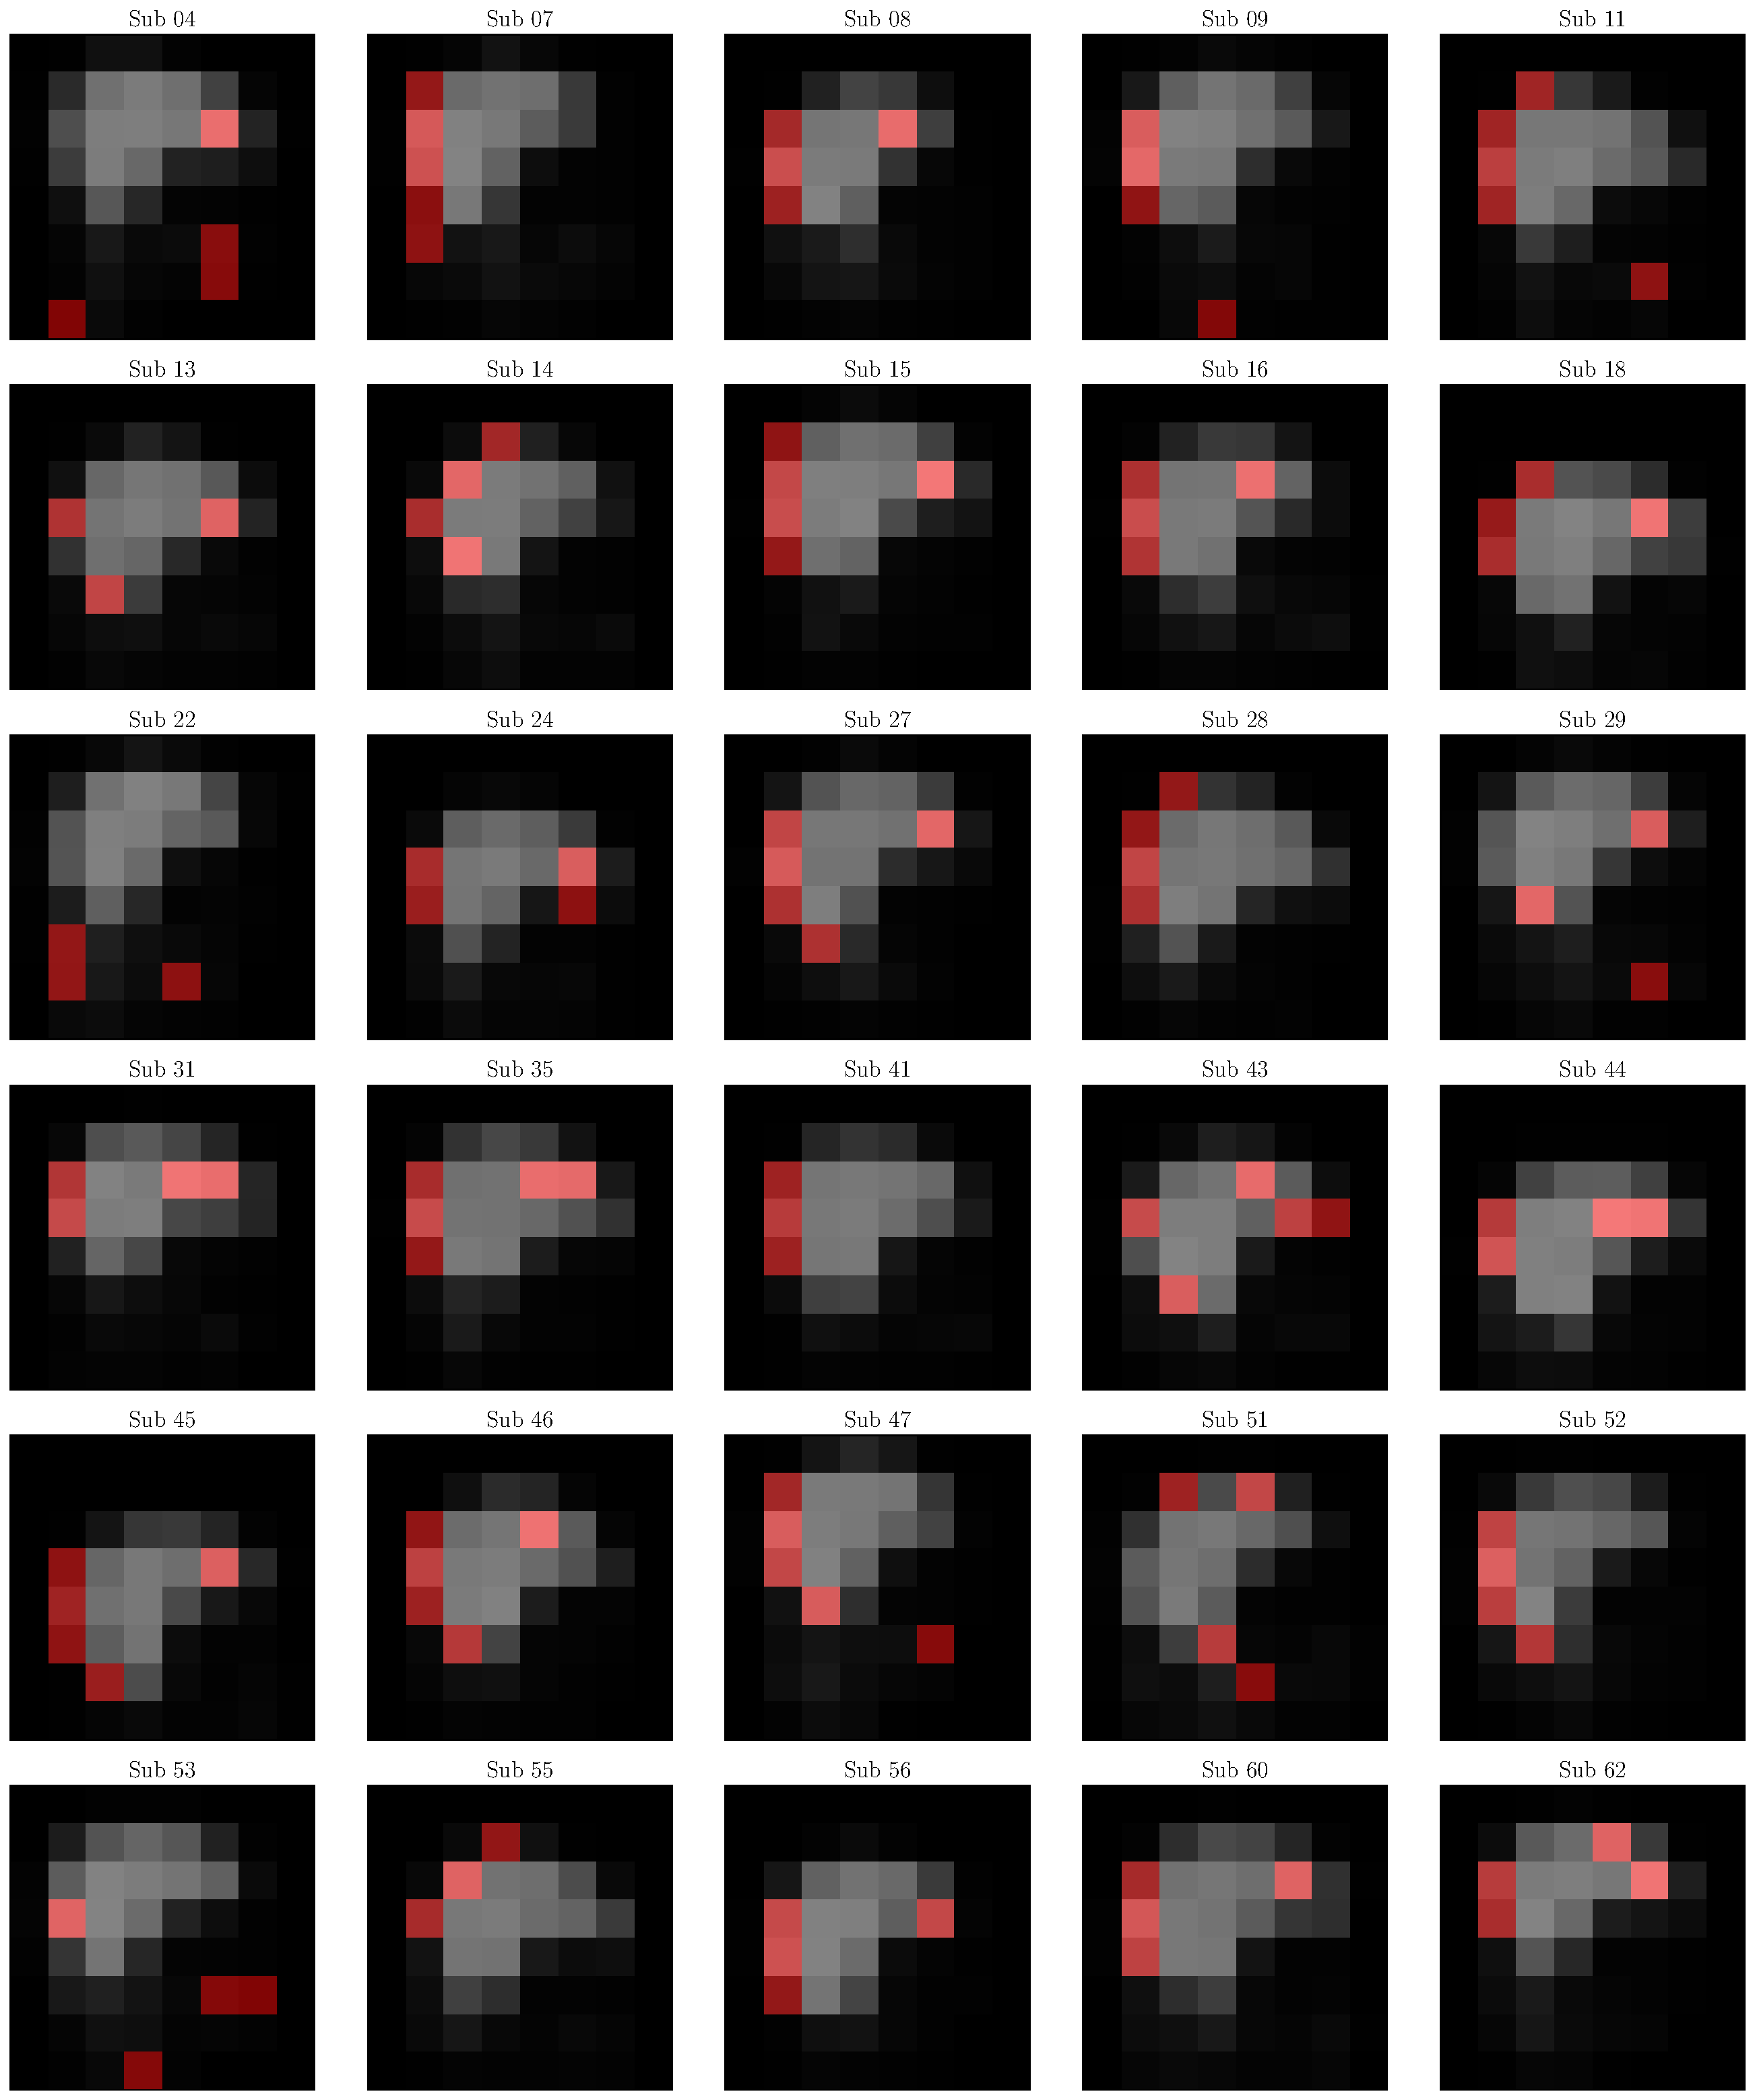
\includegraphics[width=0.8\textwidth]{cross_correlations.pdf}
    \caption{Regions of interest obtained as a result of cross-correlation analysis with the video sequence character}
\end{figure}
\begin{figure}[h!]
    \centering
    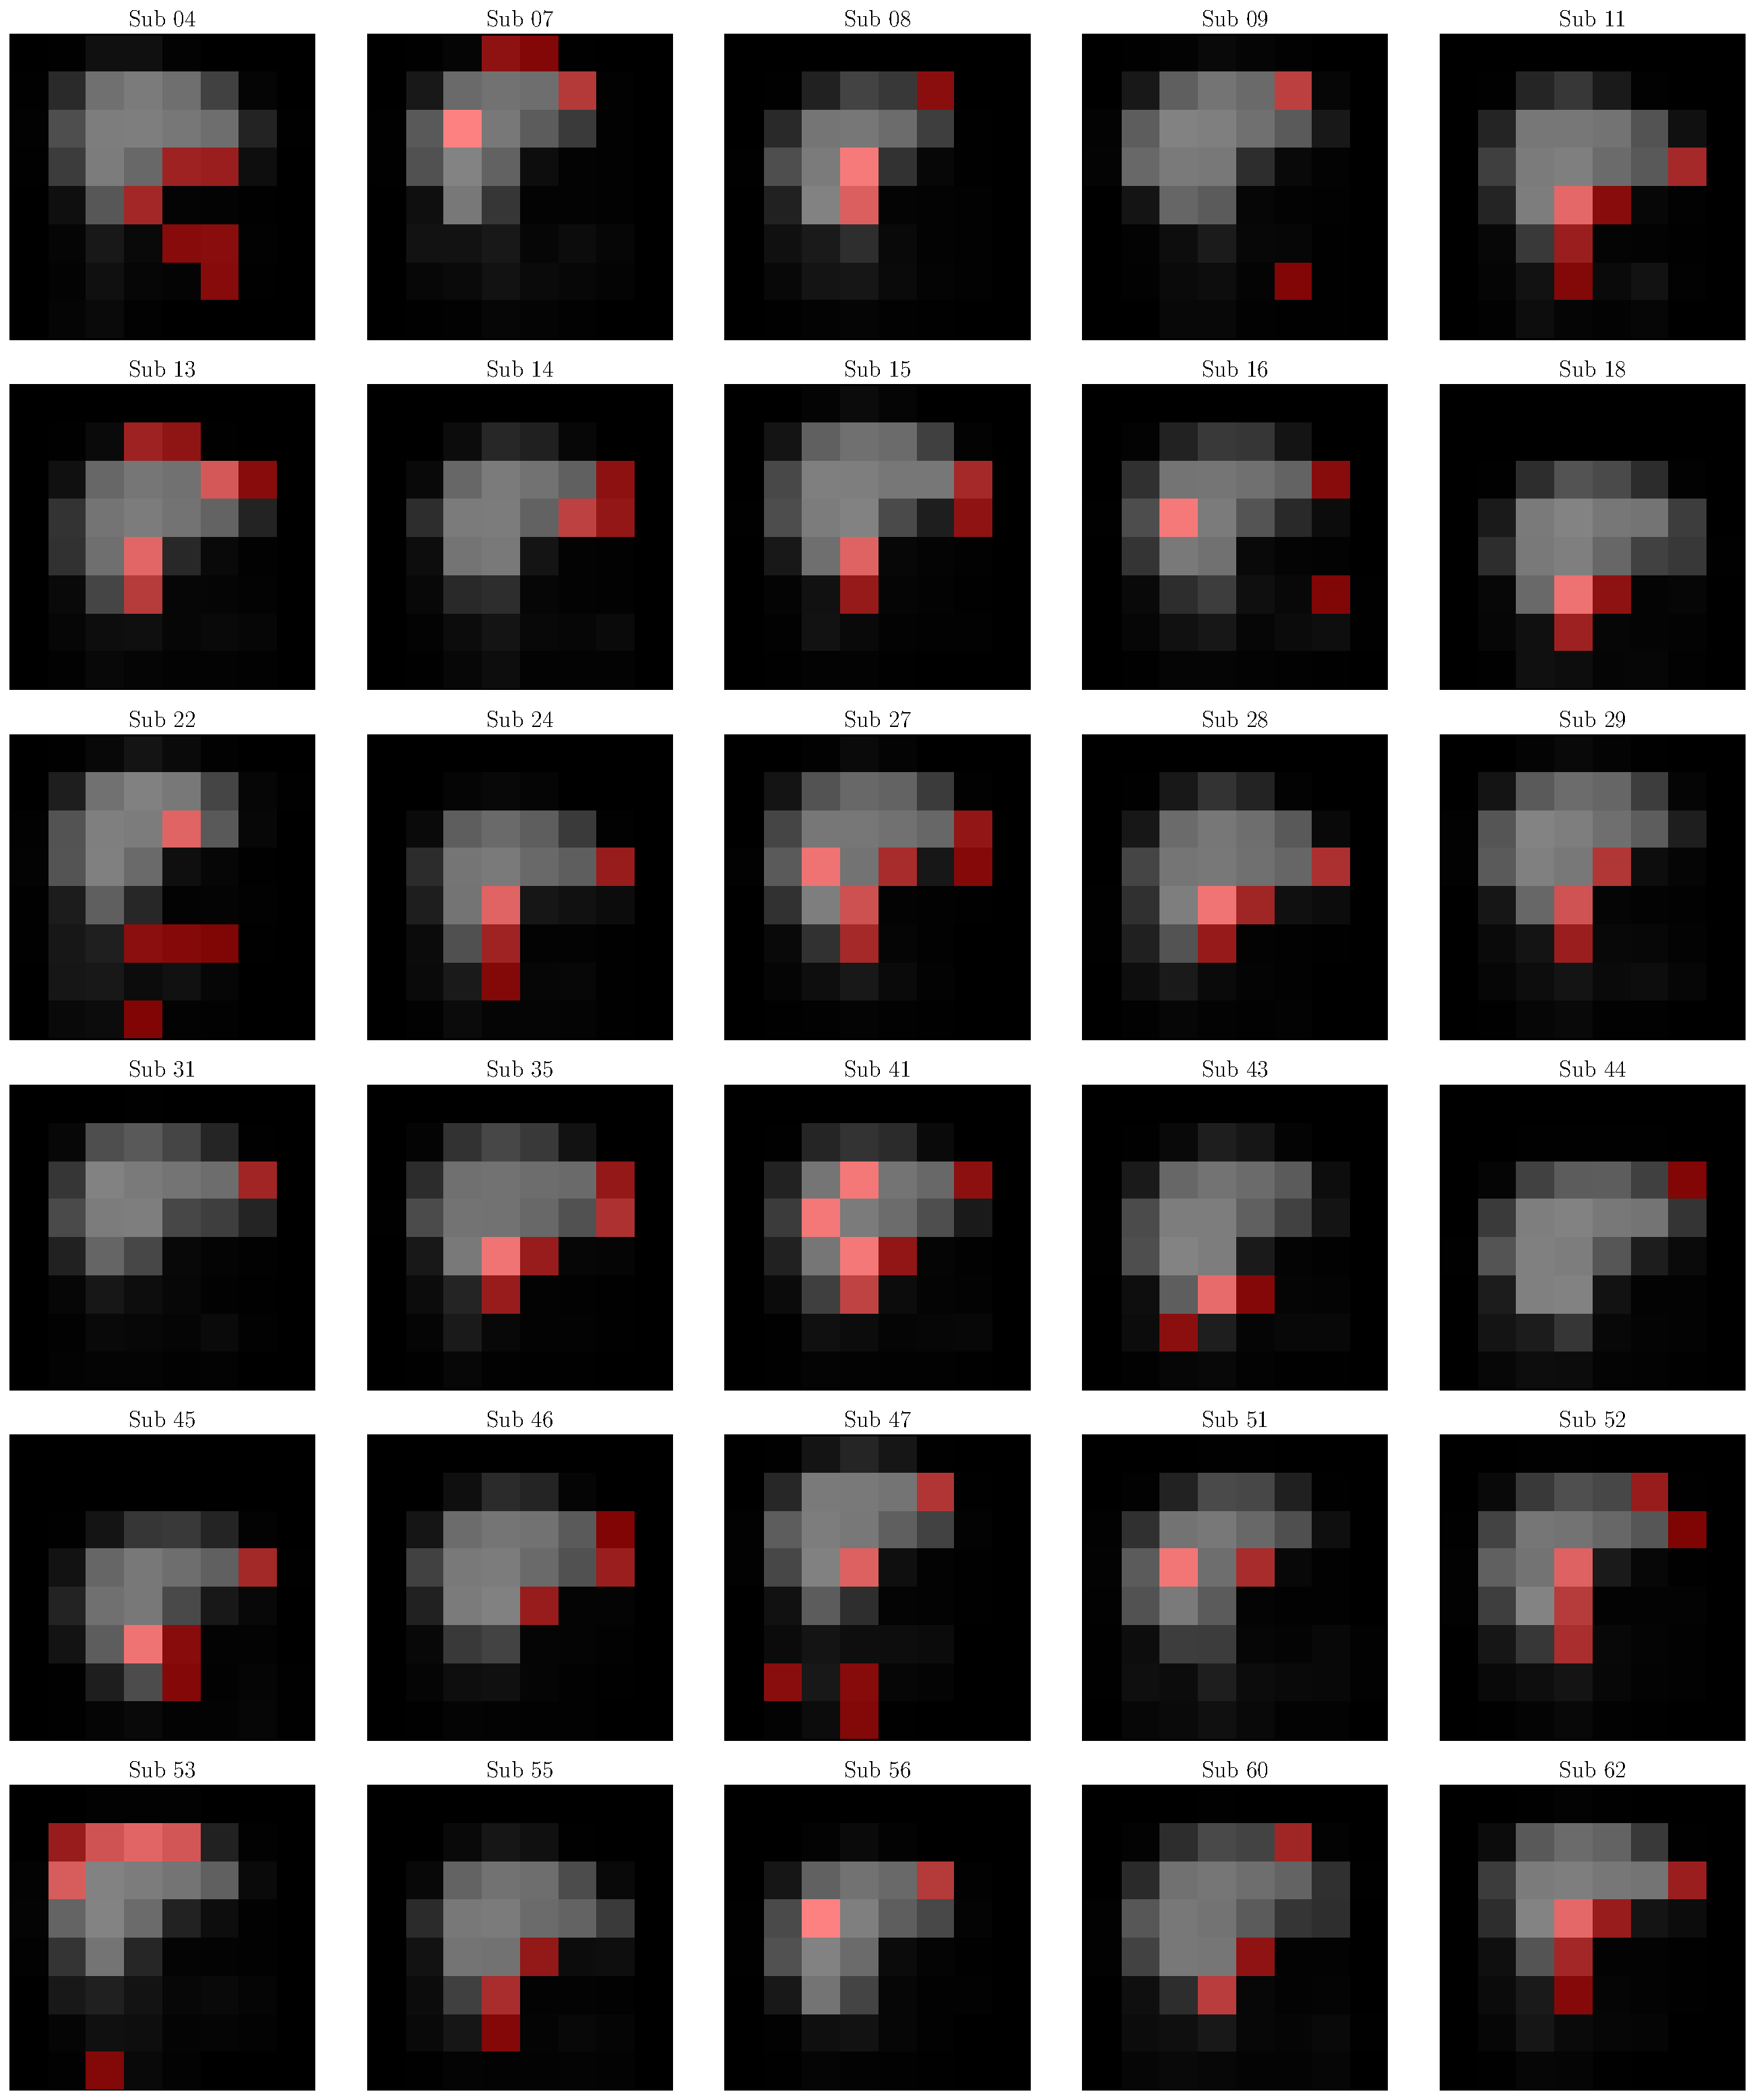
\includegraphics[width=0.8\textwidth]{cross_correlations_trash.pdf}
    \caption{Regions of interest obtained as a result of cross-correlation analysis with noise}
\end{figure}



\section{Вычислительный эксперимент}
\subsection{EEG Motor Movement/Imagery Dataset}
Для анализа работоспособности предложенного метода, а также проверки гипотез
проведен вычислительный эксперимент.
Для проведения исследования используется набор данных Physionet \citep{schalk2004bci2000, EEG_MI} для классификации ЭЭГ сигналов 
двигательных активностей, моторных образов. 
Записи были получены от 109 испытуемых с использованием системы BCI2000 и получены с 64 электродов в системе 10-10 \citep{seeck2017standardized} 
с частотой дискретизации 160 Гц. 
Каждый испытуемый выполнил 14 пробежек, включая две базовые пробежки, одну с открытыми глазами, а другую с закрытыми, 
каждая продолжительностью в одну минуту. После этих базовых пробежек они выполнили четыре различных задания, каждое из которых повторялось по три раза, 
причем каждое задание длилось две минуты.
 
Для проведения базового эксперимента используется подвыборка для задачи бинарной классификации состояния глаз открыты/закрыты.

\subsection*{Применение Римановой геометрии}
Используем подвыборку для классификации состояния глаз открыты/закрыты.
Рассмотрим несколько классических методов классификации. 
Метод опорных векторов~---один из наиболее популярных методов обучения, который применяется для решения задач классификации и регрессии.
Чтобы показать преимущество перехода к Риманову касательному пространству, проведем следующий эксперимент. 
Векторизуем все многомерные временные ряды и обучим на полученных векторах SVM. 
Теперь применим алгоритм векторизации Tangent Space Mapping (TSM) на многомерных временных рядах и после этого обучим SVM на векторизованных данных. 
Результаты на валидации и тесте приведены в таблице \ref{table:Riman}. 
Качество классификации после проектирования на касательное пространство гораздо лучше.

\begin{table}[h!]
	\centering
	\caption{Сравнение методов}
	\begin{tabular}{|c|c|c|}
		\hline
		& \multicolumn{2}{|c|}{accuracy}  \\ \hline 
		Метод & валидация  & тест \\ \hline \hline
		SVM    & $0.732$ & $0.697$      \\ \hline
		TSM SVM    & $0.939$ & $0.954$		\\ \hline
	\end{tabular}
	\label{table:Riman}
\end{table}



\subsection{UCI EEG Eye State}
Набор данных бинарной классификации состояния глаз получен в результате одного непрерывного измерения неинвазивного ЭЭГ с 
помощью нейроголовки Emotiv EEG с использованием 14 датчиков, на рис.\ref{fig:1} задействованные датчики
изображены красным цветом. 
\begin{figure}[h]
	\centering
	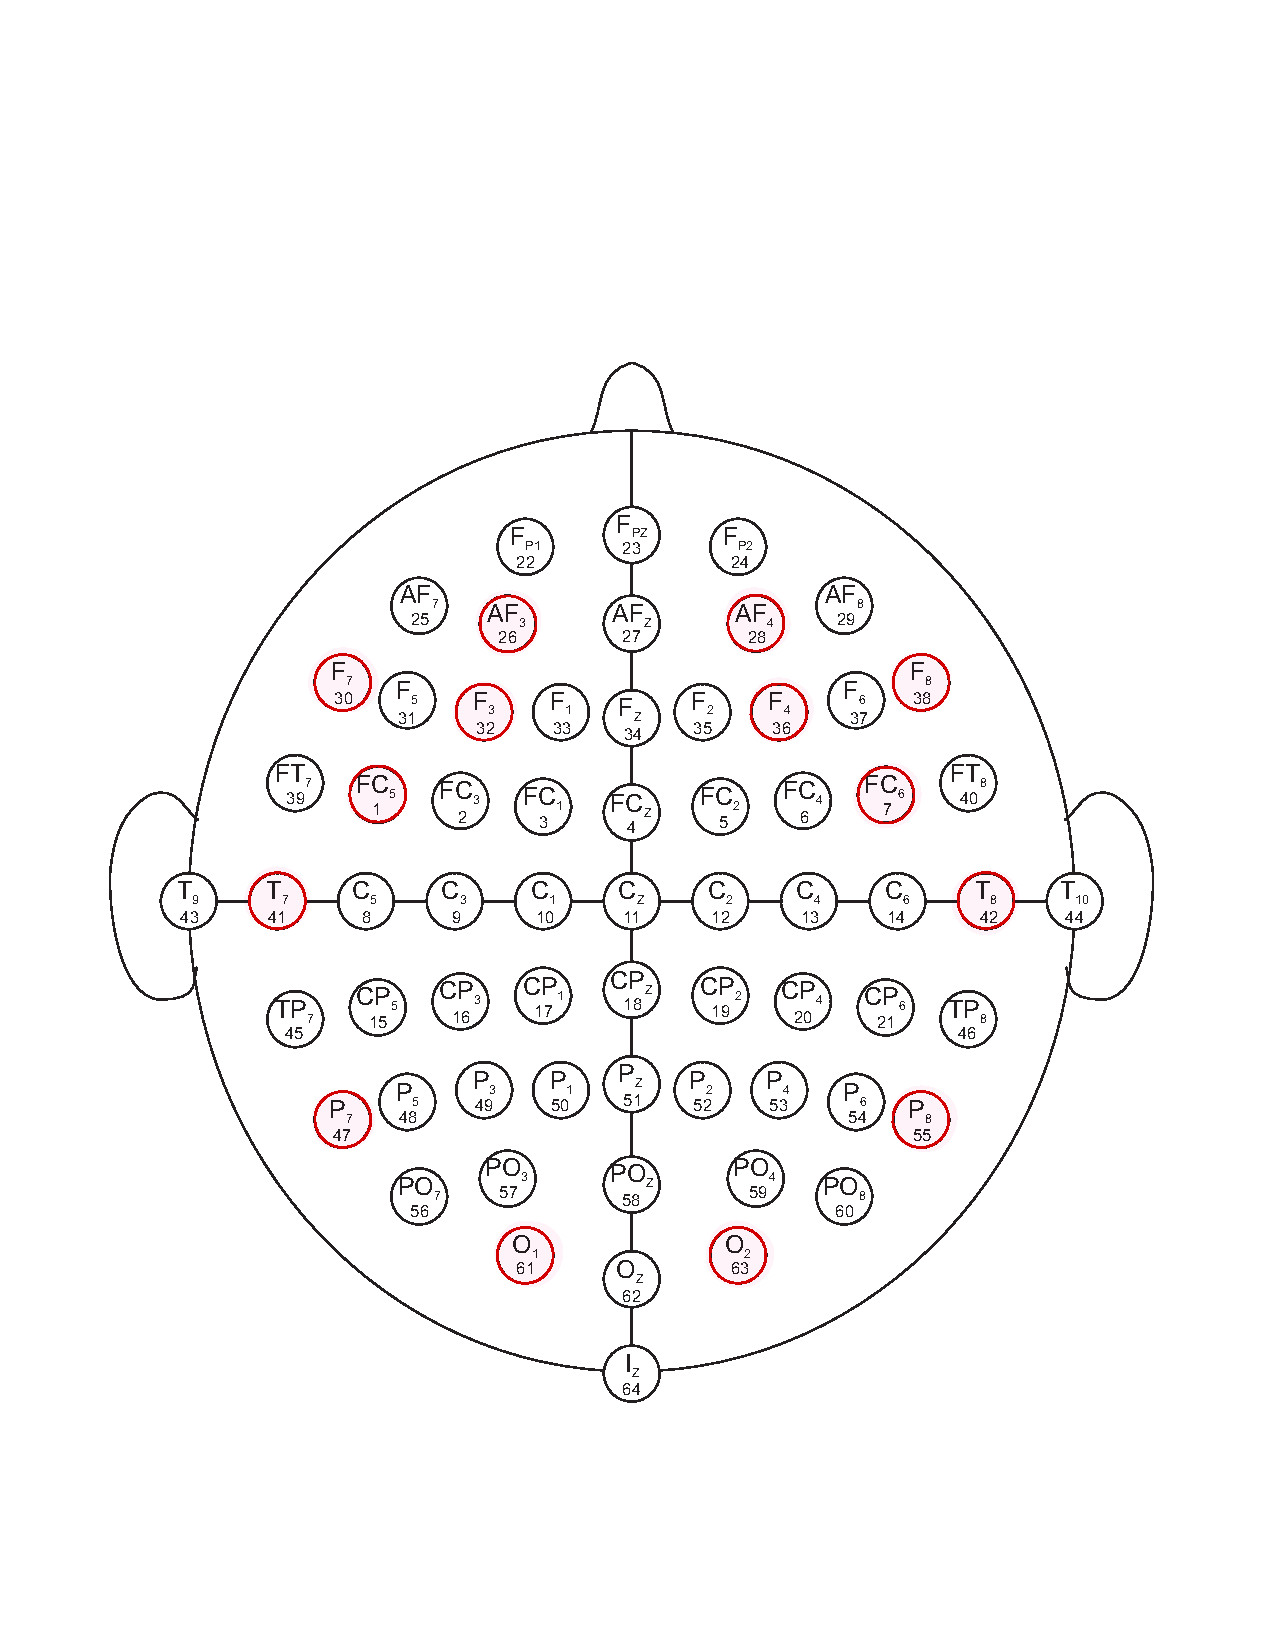
\includegraphics[width=0.75\textwidth]{64_channel_sharbrough.pdf}
	\caption{Задействованные датчики ЭЭГ при измерении сигнала}
	\label{fig:1}
\end{figure}


Продолжительность измерения в выборке составила 117 секунд. 
Состояние глаз было зафиксировано с помощью камеры во время измерения ЭЭГ и позже добавлено 
вручную в файл после анализа видеокадров. Метка <<1>> указывает на состояние с закрытыми глазами, а 
<<0>> ~--- на состояние с открытыми глазами. Все значения приведены в хронологическом порядке с 
первым измеренным значением в верхней части данных.
Основные характеристики выборки представлены в
Таблице~\ref{table:sample}.

\begin{table}
	\centering
	\caption{Описание выборки}
	\begin{tabular}{|c|c|c|}
		\hline
		Название                       & Обозначение & Значение             \\
		\hline \hline
		Продолжительность обследования & $\tau$         & 117 с                \\ \hline
		Частота измерения сигнала      & $\mu$       & 128.03 $\text{с}^{-1}$   \\ \hline
	    Число каналов (датчиков)    & $K$   & 14          \\ \hline
		Число измерений сигнала             & $T$  & 14980           \\ \hline
	\end{tabular}
	\label{table:sample}
\end{table}

\section{Заключение}


\newpage

\bibliographystyle{plain}
\bibliography{references.bib}

\end{document}
